\documentclass{article}
\usepackage[hyphens]{url}
\usepackage{mathtools}
\usepackage{amsmath}
\usepackage{listings}
\usepackage{graphicx}
\usepackage[margin=1in]{geometry}
\usepackage{float}
\floatstyle{boxed}
\restylefloat{figure}
\lstset{basicstyle=\footnotesize, breaklines=true}
\begin{document}


\title{CS595 Intro to Web Science, Assignment \#8}
\author{Valentina Neblitt-Jones}
\date{November 14, 2013}
\maketitle

\newpage
\listoftables
\lstlistoflistings
\listoffigures

\newpage
\section*{Instructions}

The goal of this project it is to use the basic recommendation principles we have learned for user-collected data. You will modify the code given to you which performs movie recommendations from the MovieLense data sets. \\

The MovieLense data sets were collected by the GroupLens Research Project at the University of Minnesota during the seven-month period from September 19th, 1997 through April 22, 1998. It is available for download from \url{http://www.grouplens.org/node/73} \\

There are three files which we will use: 

\subsection*{u.data}

u.data: 100,000 ratings by 943 users on 1,682 movies. Each user has rated at least 20 movies. Users and items are numbered consecutively from 1. The data is randomly ordered. This is a tab-separated list of user id, item id, rating, and timestamp. \\

The time stamps are unix seconds since 1/1/1970 UTC. \\

Example: 

\begin{table}[!h]
\centering
\begin{tabular}{c c c c}
user id & item id &  rating & timestamp \\
\hline
196 & 242 & 3 & 881250949 \\
186 & 302 & 3 & 891717742 \\
22 & 377 & 1 & 878887116 \\
244 & 51 & 2 & 880606923 \\
166 & 346 & 1 & 886397596 \\
298 & 474 & 4 & 884182806 \\
115 & 265 & 2 & 881171488 \\
\end{tabular}
\end{table}

\subsection*{u.item}

u.item: Information about the 1,682 movies. This is a tab separated list of movie id, movie title, release date, video release date, IMDb URL, unknown, Action, Adventure, Animation, Children's, Comedy, Crime, Documentary, Drama, Fantasy, Film-Noir, Horror, Musical, Mystery, Romance, Sci-Fi, Thriller, War, and Western. \\

The last 19 fields are the genres, a 1 indicates the movie is of that genre, a 0 indicates it is not; movies can be in several genres at once. The movie ids are the ones used in the u.data set. \\

Example: \\

\begin{verbatim}
161|Top Gun (1986)|01-Jan-1986||http://us.imdb.com/M/title-exact?Top\%20Gun\%20(1986)
|0|1|0|0|0|0|0|0|0|0|0|0|0|0|1|0|0|0|0 
162|On Golden Pond (1981)|01-Jan-1981||
http://us.imdb.com/M/title-exact?On\%20Golden\%20Pond\%20(1981)
|0|0|0|0|0|0|0|0|1|0|0|0|0|0|0|0|0|0|0 
163|Return of the Pink Panther, The (1974)|01-Jan-1974||
http://us.imdb.com/M/title-exact?Return\%20of\%20the\%20Pink\%20Panther,\%20The\%20(1974)
|0|0|0|0|0|1|0|0|0|0|0|0|0|0| 0|0|0|0|0
\end{verbatim}

\subsection*{u.user}

u.user: Demographic information about the users. This is a tab-separate list of user id, age, gender, occupation, and zip code. \\

Example: \\

\begin{table}[!h]
\centering
\begin{tabular}{c c c c c}
user id & age &  gender & occupation & zip code \\
\hline
1 & 24 & M & technician & 85711 \\
2 & 53 & F & other & 94043 \\
2 & 23 & M & writer & 32067 \\
4 & 24 & M & technician & 43537 \\
5 & 33 & F & other & 15213 \\
\end{tabular}
\end{table}

The code for reading from the u.data and u.item files and creating recommendations is described in the book Programming Collective Intelligence (check mail for more details). You are to modify recommendations.py to answer the following questions. Each question your program answers correctly will award you 10 points. You must have the question answered completely correct; partial credit will be only awarded if your answer is very close to the correct one. Your output should clearly indicate the answers from the question you answered. Provide any relevant discussion.



\newpage
\section*{Answers}
\renewcommand\thesubsection{\arabic{subsection}}
\subsection{What 5 movies have the highest average ratings? Show the movies and their ratings sorted by their average ratings.}

\begin{table}[!h]
\centering
\begin{tabular}{l c}
Movie Title & Average Rating \\
\hline
Santa with Muscles (1996) & 5.0  \\
Star Kid (1997) & 5.0  \\
They Made Me a Criminal (1939) & 5.0  \\
Aiqing wansui (1994) & 5.0  \\
Marlene Dietrich: Shadow and Light (1996) & 5.0  \\
A Great Day in Harlem (1994) & 5.0  \\
Entertaining Angels: The Dorothy Day Story (1996) & 5.0  \\
Someone Else's America (1995) & 5.0  \\
Prefontaine (1997) & 5.0  \\
The Saint of Fort Washington (1993) & 5.0  \\
\hline
\end{tabular}
\caption{Movies with the Highest Average Rating}
\end{table}

The output from my program produced 10 movies with the highest average score. I created dictionaries to hold movie ratings, average ratings, movie information and finally the top movies. This problem required use of mostly u.data since it had the ratings and the movie IDs, but also u.item so that the movie IDs could be referenced by their titles.

So I read in the u.data file and in my loop I placed the ID and the rating in the dictionary. If the dictionary already had the ID, then I only appended the rating. After this dictionary was created, I iterated through the new dictionary and calculated the mean score of the ratings associated with each key. I found a question/answer in Stack Overflow that suggested using numpy library and its mean function \cite{numpymean}. The resulting list had the data I desired, but in order by movie ID. Since dictionaries inherently sort this way, I had to find a way to produce the same list in reverse order by average rating and used a solution provided in a Stack Overflow answer. \cite{dictsortvalue} This sorted on the average rating value and placed the result in a dictionary called top movies.

I was having a problem reading in u.item and receiving an error starting with ``UnicodeDecodeError: 'utf8' codec can't decode ...''. This required using the codecs library \cite{codecs} so I could specify how it should be read.

\begin{lstlisting}[frame=single, caption=highestavgrating.py, label=highaverage]
import datetime
import numpy
import codecs

g = open('highestaveragerating.txt', 'w')

movieratings={}
averageratings={}
movieinfo={}
topmovies={}

with open('/Users/vneblitt/Documents/cs595-f13/assignment08/dataset/u.data', 'r') as f:
	movieratinginfo = f.readlines()
	for line in movieratinginfo:
		(userid, itemid, rating, timestamp) = line.split('\t')
		if itemid in movieratings:
			movieratings[itemid].append(int(rating))
		else:
			movieratings[itemid] = [int(rating)]
f.close()

for movie in movieratings:
	ratings = movieratings[movie]
	average = numpy.mean(ratings)
	averageratings[movie] = average

#stack overflow http://stackoverflow.com/questions/613183/python-sort-a-dictionary-by-value (11/10/2013)
for movieid in sorted(averageratings, key=averageratings.get, reverse=True)[0:10]:
	topmovies[movieid] = averageratings[movieid]

with (codecs.open('/Users/vneblitt/Documents/cs595-f13/assignment08/dataset/u.item','r', 'iso-8859-1')) as h:
	moviedata = h.readlines()
	for line in moviedata:
		(movieid, movietitle) = line.split('|')[0:2]
		movieinfo[movieid] = movietitle
h.close()

for movie in topmovies:
	g.write(movieinfo[movie] + ' ' + str(topmovies[movie]) + '\n')

g.close()
\end{lstlisting}

%\begin{lstlisting}[frame=single, caption=highestavgrating.py, label=highaverage]
%\end{lstlisting}

\newpage
\subsection{What 5 movies have received the most ratings? Show the movies and the number of ratings sorted by number of ratings.}

\begin{table}[!h]
\centering
\begin{tabular}{l c}
Movie Title & No. of Ratings \\
\hline
Star Wars (1977) & 583  \\
Contact (1997) & 509  \\
Fargo (1996) & 508  \\
Return of the Jedi (1983) & 507  \\
Marlene Dietrich: Shadow and Light (1997) & 485  \\
\hline
\end{tabular}
\caption{Movies with the Most Ratings}
\end{table}

The output from my program produced the desired quantity of 5 movies. I created dictionaries to hold movie ratings, counted ratings, and movie information. This problem also required use of mostly u.data since it had the ratings and the movie IDs, but also u.item so that the movie IDs could be referenced by their titles.

This program was similar to Q1 except that after the first dictionary was created, I iterated through it and used the length of a list function to calculated the number of ratings for each movie. I did not have a ``too many results'' problem this time. this is because it is less likely that raters would have rated the exact same number of movies.

\begin{lstlisting}[frame=single, caption=mostratings.py, label=mostratings]
[...]
for movie in movieratings:
	ratings = movieratings[movie]
	ratingscount = len(ratings)
	countingratings[movie] = ratingscount
#print(countingratings)

[...]

#stack overflow http://stackoverflow.com/questions/613183/python-sort-a-dictionary-by-value (11/10/2013)
for movieid in sorted(countingratings, key=countingratings.get, reverse=True)[0:5]:
	g.write(movieinfo[movieid] + ' ' + str(countingratings[movieid]) + '\n')

g.close()
\end{lstlisting}

\newpage
\subsection{What 5 movies were rating the highest on average by women? Show the movies and their ratings sorted by ratings.}

\begin{table}[!h]
\centering
\begin{tabular}{l c}
Movie Title & Average Rating \\
\hline
Stripes (1981) & 5.0  \\
Mina Tannenbaum (1994) & 5.0  \\
Faster Pussycat! Kill! Kill! (1965) & 5.0  \\
Foreign Correspondent (1997) & 5.0  \\
Telling Lies in America (1996) & 5.0  \\
Maya Lin: A Strong Clear Vision (1994) & 5.0  \\
Prefontaine (1997) & 5.0  \\
Someone Else's America (1995) & 5.0  \\
Everest (1998) & 5.0  \\
Year of the Horse (1997) & 5.0  \\
The Visitors (Les Visiteurs) (1993) & 5.0 \\
\hline
\end{tabular}
\caption{Movies with the Highest Average Rating By Women}
\end{table}

The output from my program produced 11 movies with the highest average rating by women. I created dictionaries to hold user information, movie ratings, average ratings, movie information and also a list to hold just the female users. This problem required use of u.data and u.item like the previous problems, but added the need for u.user.

So I read in the u.user file and in my loop I placed the userid, age and gender. I did not need age for this problem, but it was in-between userid and gender which I did need. The resulting dictionary held the userid as a key and the gender as a value. Next, I created a list of userid that only held the IDs of women. The movieratings dictionary creation involved checking if the userid was in the list of women first. Then checking if the woman's userid was already in the dictionary. If it was, it appended the rating to her key. If not it created the key and rating. Next it calculated the average rating and sorted by average rating as it had in Q1. 

\begin{lstlisting}[frame=single, caption=highestwomen.py, label=highwomen]
import codecs
import numpy

g = open('highestwomen.txt', 'w')

userinfo={}
theladies=[]
movieratings={}
averageratings={}
movieinfo={}


# Parse u.user to get the userid, age, and gender (only need userid and gender)
with open('/Users/vneblitt/Documents/cs595-f13/assignment08/dataset/u.user', 'r') as j:
	userdata = j.readlines()
	for line in userdata:
		(userid, age, gender) = line.split('|')[0:3]
		userinfo[userid] = gender

# Create a list of userids that only belong to women
for user in userinfo:
	if userinfo[user] == 'F':
		theladies.append(user)

# Create a dictionary of movies and ratings only if the user is a woman
with open('/Users/vneblitt/Documents/cs595-f13/assignment08/dataset/u.data', 'r') as f:
	movieratinginfo = f.readlines()
	for line in movieratinginfo:
		(userid, itemid, rating, timestamp) = line.split('\t')
		if userid in theladies:
			if itemid in movieratings:
				movieratings[itemid].append(int(rating))
			else:
				movieratings[itemid] = [int(rating)]
f.close()

# Calculate the average rating for each movie
for movie in movieratings:
	ratings = movieratings[movie]
	average = numpy.mean(ratings)
	averageratings[movie] = average

with (codecs.open('/Users/vneblitt/Documents/cs595-f13/assignment08/dataset/u.item','r', 'iso-8859-1')) as h:
	moviedata = h.readlines()
	for line in moviedata:
		(movieid, movietitle) = line.split('|')[0:2]
		movieinfo[movieid] = movietitle
h.close()

#stack overflow http://stackoverflow.com/questions/613183/python-sort-a-dictionary-by-value (11/10/2013)
for movieid in sorted(averageratings, key=averageratings.get, reverse=True)[0:11]:
	g.write(movieinfo[movieid] + ' ' + str(averageratings[movieid]) + '\n')

g.close()
\end{lstlisting}

\newpage
\subsection{What 5 movies were rated the highest on average by men? Show the movies and their ratings sorted by ratings.}

\begin{table}[!h]
\centering
\begin{tabular}{l c}
Movie Title & Average Rating \\
\hline
A Great Day in Harlem (1994) & 5.0 \\
Delta of Venus (1994) & 5.0 \\
Love Serenade (1996) & 5.0 \\
They Made Me a Criminal (1939) & 5.0 \\
Hugo Pool (1997) & 5.0 \\
A Letter From Death Row (1998) & 5.0 \\
Prefontaine (1997) & 5.0 \\
Santa with Muscles (1996) & 5.0 \\
The Saint of Fort Washington (1993) & 5.0 \\
Star Kid (1997) & 5.0 \\
Aiqing wansui (1994) & 5.0 \\
The Leading Man (1996) & 5.0 \\
The Quiet Room (1996) & 5.0 \\
Marlene Dietrich: Shadow and Light (1996)  & 5.0 \\
Little City (1998) & 5.0 \\
Entertaining Angels: The Dorothy Day Story (1996) & 5.0 \\
\hline
\end{tabular}
\caption{Movies with the Highest Average Rating By Men}
\end{table}

The output from my program produced 16 movies with the highest average rating by men. The solution was identical to Q3 except that I created a list of userids belonging to men to derive movierating info dictionary.

\begin{lstlisting}[frame=single, caption=highestmen.py, label=highmen]
import codecs
import numpy

g = open('highestmen.txt', 'w')

userinfo={}
theguys=[]
movieratings={}
averageratings={}
movieinfo={}


[...]

# Create a list of userids that only belong to women
for user in userinfo:
	if userinfo[user] == 'M':
		theguys.append(user)

# Create a dictionary of movies and ratings only if the user is a man
with open('/Users/vneblitt/Documents/cs595-f13/assignment08/dataset/u.data', 'r') as f:
	movieratinginfo = f.readlines()
	for line in movieratinginfo:
		(userid, itemid, rating, timestamp) = line.split('\t')
		if userid in theguys:
			if itemid in movieratings:
				movieratings[itemid].append(int(rating))
			else:
				movieratings[itemid] = [int(rating)]
f.close()

[...]

g.close()
\end{lstlisting}

%\begin{lstlisting}[frame=single, caption=highestavgrating.py, label=highaverage]
%\end{lstlisting}

\newpage
\subsection{What movie received ratings most like Top Gun? Which movie received ratings that were least like Top Gun (negative correlation)?}

\begin{figure}[H]
\centering
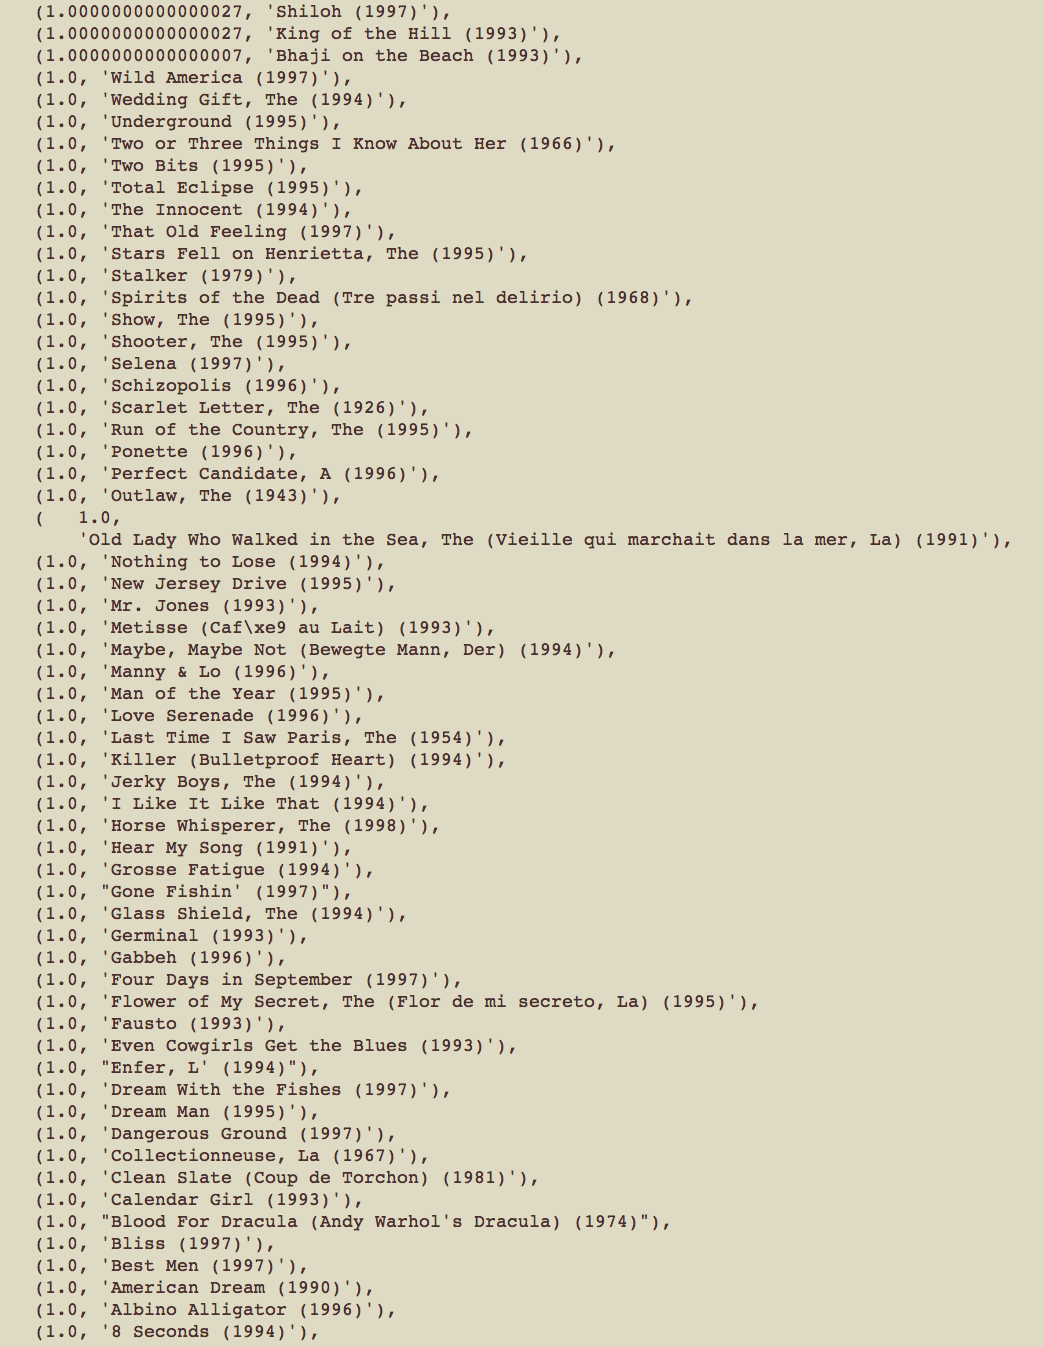
\includegraphics[scale=0.40]{q05/mostliketopgun}
\caption{Movies Most Like Top Gun}
\label{mostliketopgun}
\end{figure}

\begin{figure}[H]
\centering
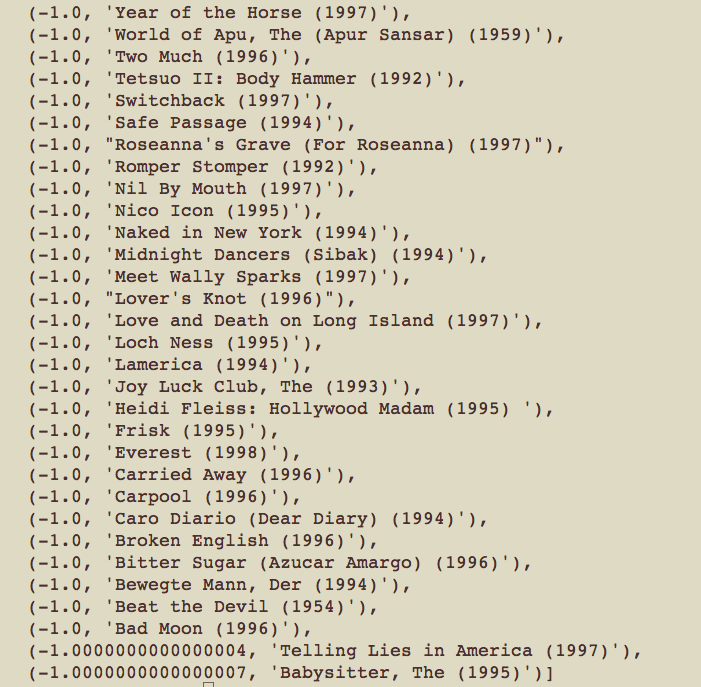
\includegraphics[scale=0.50]{q05/leastliketopgun}
\caption{Movies Least Like Top Gun}
\label{leastliketopgun}
\end{figure}

I used recommendations.py (Listing \ref{recommendations}) as a library. Since it was not using Python 3.3, I switched to Python 2.x for this question. I used loadMovieLens to load the dataset. Since I did this one near the end, I did not know about this handy way to load and parse the data. It did not have the codecs problem that I ran into with Python 3.3 either. Though I did notice some odd title behavior when I reviewed ``prefs'' in the terminal. Next I ran the calculateSimilarItems function in recommendations.py. Originally, I ran it `as is', but discussion on this question and the reading indicated that similarity should be changed to sim\_pearson since it is more precise than Euclidean distance. \cite{pci}

I got the same output as was discussed in the class email list. Three movies had values greater than 1 (Figure \ref{mostliketopgun}) and two movies had values less than -1 (Figure \ref{leastliketopgun}). I tried using rounding as suggested by a classmate. It ``fixed'' the two that were less than -1, but the three that were greater than 1 remained. I did decide to treat them all as ties.

Based on what I know about many of the movies that received ratings most similar to Top Gun, I would not be able to solely use this data to recommend a movie to a customer when I worked at Blockbuster. For instance, it is likely that someone who liked Bhaji on the Beach would like Top Gun, the reverse it not likely true. Top Gun is a successful movie seen and enjoyed by a general audience. Bhaji on the Beach, however, is a foreign independent movie that would be liked by the same audience that would frequent by the Naro Cinema in Ghent.

\begin{lstlisting}[frame=single, caption=topgun01.py, label=topgun]
import sys
import pprint

sys.path.insert(0, '/Users/vneblitt/Documents/cs595-f13/assignment08/library')

import recommendations

g = open('topgun.txt', 'w')

prefs = recommendations.loadMovieLens(path='/Users/vneblitt/Documents/cs595-f13/assignment08/dataset')

answer = recommendations.calculateSimilarItems(prefs,n=1664)

pp = pprint.PrettyPrinter(indent=4)

pp.pprint(answer['Top Gun (1986)'])

g.write(str(answer))
g.close()

\end{lstlisting}

\newpage
\subsection{Which 5 raters rated the most films? Show the raters' IDs and the number of films each rated.}

\begin{table}[!h]
\centering
\begin{tabular}{l c}
Rater ID & No. of Ratings \\
\hline
405 & 737  \\
655 & 685  \\
13 & 636  \\
450 & 540  \\
276 & 518  \\
\hline
\end{tabular}
\caption{Raters Who Rated the Most Films}
\end{table}

This question was a little closer related to Q2. The output from my program produced the desired quantity of 5 raters. I created dictionaries to hold movie raters, counted ratings, and top raters. This problem required use of u.data only since it had the ratings and the raters. We could not get the raters' name from any file and the movie titles were also not necessary.

This program was similar to Q2 except that I created a dictionary of movie raters and their ratings. I iterated through it and used the length of a list function to calculated the number of ratings for each rater.  The dictionary of top raters was produced by sorting on value and producing a reverse order list. Again, I did not have a ``too many results'' problem this time. this is because it is less likely that raters would have rated the exact same number of movies.


\begin{lstlisting}[frame=single, caption=prolificraters.py, label=prolificraters]
g = open('prolificraters.txt', 'w')

movieraters={}
countingratings={}
topraters={}

with open('/Users/vneblitt/Documents/cs595-f13/assignment08/dataset/u.data', 'r') as f:
	movieratinginfo = f.readlines()
	for line in movieratinginfo:
		(userid, itemid, rating, timestamp) = line.split('\t')
		if userid in movieraters:
			movieraters[userid].append(int(rating))
		else:
			movieraters[userid] = [int(rating)]
f.close()
#print(movieraters)

for rater in movieraters:
	ratings = movieraters[rater]
	ratingscount = len(ratings)
	countingratings[rater] = ratingscount
#print(countingratings)

g.write('rater id, ' + 'number of ratings' + '\n')

#stack overflow http://stackoverflow.com/questions/613183/python-sort-a-dictionary-by-value (11/10/2013)
for rater in sorted(countingratings, key=countingratings.get, reverse=True)[0:5]:
	topraters[rater] = countingratings[rater]
	g.write(rater + ', ' + str(countingratings[rater]) + '\n')

g.close()
\end{lstlisting}

\newpage
\subsection{Which 5 raters most agreed with each other? Show the raters' IDs and Pearson's r, sorted by r.}

\newpage
\subsection{Which 5 raters most disagreed with each other (negative correlation)? Show the raters' IDs and Pearson's r, sorted by r.}

\newpage
\subsection{What movie was rated highest on average by men over 40? By men under 40?}

\begin{table}[!h]
\centering
\begin{tabular}{l c}
Movie Title & Average Rating \\
\hline
The World of Apu (Apur Sansar) (1959) & 5.0 \\
Indian Summer (1996) & 5.0 \\
Star Kid (1997) & 5.0 \\
Hearts and Minds (1996) & 5.0 \\
Marlene Dietrich: Shadow and Light (1996)  & 5.0 \\
Aparajito (1956) & 5.0 \\
A Great Day in Harlem (1994) & 5.0 \\
Strawberry and Chocolate (Fresa y chocolate) (1993) & 5.0 \\
Unstrung Heroes (1995) & 5.0 \\
Prefontaine (1997) & 5.0 \\
Faithful (1996) & 5.0 \\
Late Bloomers (1996) & 5.0 \\
Double Happiness (1994) & 5.0 \\
The Leading Man (1996) & 5.0 \\
They Made Me a Criminal (1939) & 5.0 \\
Little City (1998) & 5.0 \\
The Little Princess (1939) & 5.0 \\
Grateful Dead (1995) & 5.0 \\
Solo (1996) & 5.0 \\
Two or Three Things I Know About Her (1966) & 5.0 \\
Rendezvous in Paris (Les Rendez-vous de Paris) (1995) & 5.0 \\
Spice World (1997) & 5.0 \\
Poison Ivy II (1995) & 5.0 \\
Boxing Helena (1993) & 5.0 \\
Ace Ventura: When Nature Calls (1995) & 5.0 \\
\hline
\end{tabular}
\caption{Movies with the Highest Average Rating By Men Over 40}
\end{table}

This solution (Listing \ref{highestmenover40}) was built on Q3 where we already had to exclude based on gender. Now we are asked to add age as a factor. I read in the file and created a list of just men over 40 at the same time. Then I  created the movierating dictionary based on whether the userid was found in the list called theguys. I calculatd the average rating, mapped the movie titles to movie IDs, and reverse sorted the list the same way I had in other problems. Listing \ref{highestmenunder40} is the same as Listing \ref{highestmenover40} except that the age factor changed from greater than 40 to less than 40.

\begin{lstlisting}[frame=single, caption=highestmenover40.py, label=highestmenover40]
import codecs
import numpy

g = open('highestmenover40.txt', 'w')

theguys=[]
movieratings={}
averageratings={}
movieinfo={}


# Parse u.user to get the userid, age, and gender and create a list of userids that only contain men over 40
with open('/Users/vneblitt/Documents/cs595-f13/assignment08/dataset/u.user', 'r') as j:
	userdata = j.readlines()
	for line in userdata:
		(userid, age, gender) = line.split('|')[0:3]
		if gender == 'M':
			if int(age) > 40:
				theguys.append(userid)

# Create a dictionary of movies and ratings only if the user is a men over 40
with open('/Users/vneblitt/Documents/cs595-f13/assignment08/dataset/u.data', 'r') as f:
	movieratinginfo = f.readlines()
	for line in movieratinginfo:
		(userid, itemid, rating, timestamp) = line.split('\t')
		if userid in theguys:
			if itemid in movieratings:
				movieratings[itemid].append(int(rating))
			else:
				movieratings[itemid] = [int(rating)]
f.close()

[...]

g.close()
\end{lstlisting}

\begin{table}[!h]
\centering
\begin{tabular}{l c}
Movie Title & Average Rating \\
\hline
Angel Baby (1995) & 5.0 \\
Crossfire (1947) & 5.0 \\
Love Serenade (1996) & 5.0 \\
The Saint of Fort Washington (1993) & 5.0 \\
A Perfect Candidate (1996) & 5.0 \\
Delta of Venus (1994) & 5.0 \\
Entertaining Angels: The Dorothy Day Story (1996) & 5.0 \\
The Leading Man (1996) & 5.0 \\
Star Kid (1997) & 5.0 \\
Aiqing wansui (1994) & 5.0 \\
Santa with Muscles (1996) & 5.0 \\
The Magic Hour (1998) & 5.0 \\
The Quiet Room (1996) & 5.0 \\
Hugo Pool (1997) & 5.0 \\
Maya Lin: A Strong Clear Vision (1994) & 5.0 \\
Prefontaine (1997) & 5.0 \\
A Letter From Death Row (1998) & 5.0 \\
Love in the Afternoon (1957) & 5.0 \\
\hline
\end{tabular}
\caption{Movies with the Highest Average Rating By Men Under 40}
\end{table}

\begin{lstlisting}[frame=single, caption=highestmenunder40.py, label=highestmenunder40]
import codecs
import numpy

g = open('highestmenunder40.txt', 'w')

theguys=[]
movieratings={}
averageratings={}
movieinfo={}


# Parse u.user to get the userid, age, and gender and create a list of userids that only contain men under 40
with open('/Users/vneblitt/Documents/cs595-f13/assignment08/dataset/u.user', 'r') as j:
	userdata = j.readlines()
	for line in userdata:
		(userid, age, gender) = line.split('|')[0:3]
		if gender == 'M':
			if int(age) < 40:
				theguys.append(userid)

[...]

g.close()
\end{lstlisting}

\newpage
\subsection{What movie was rated highest on average by women over 40? By women under 40?}

\begin{table}[!h]
\centering
\begin{tabular}{l c}
Movie Title & Average Rating \\
\hline
Balto (1995) & 5.0 \\
Pocahontas (1995) & 5.0 \\
A Grand Day Out (1992) & 5.0 \\
Mary Shelley's Frankenstein (1994) & 5.0 \\
Ma vie en rose (My Life in Pink) (1997) & 5.0 \\
Bride of Frankenstein (1935) & 5.0 \\
Shall We Dance? (1937) & 5.0 \\
The Visitors (Les Visiteurs) (1993) & 5.0 \\
The Great Dictator (1940) & 5.0 \\
A Letter From Death Row (1998) & 5.0 \\
The Wrong Trousers (1993) & 5.0 \\
In the Bleak Midwinter (1995) & 5.0 \\
Best Men (1997) & 5.0 \\
Safe (1995) & 5.0 \\
Funny Face (1957) & 5.0 \\
Tombstone (1993) & 5.0 \\
Angel Baby (1995) & 5.0 \\
The Band Wagon (1953) & 5.0 \\
The Quest (1996) & 5.0 \\
The Nightmare Before Christmas (1993) & 5.0 \\
Gold Diggers: The Secret of Bear Mountain (1995) & 5.0 \\
Shallow Grave (1994) & 5.0 \\
Foreign Correspondent (1940) & 5.0 \\
Top Hat (1935) & 5.0 \\
Mina Tannenbaum (1994) & 5.0 \\
Swept from the Sea (1997) & 5.0 \\
\hline
\end{tabular}
\caption{Movies with the Highest Average Rating By Women Over 40}
\end{table}

This solution (Listing \ref{highestwomenover40}) was built on Q9 where we already had to exclude based on gender and age. Listing \ref{highwomenunder40} is the same as Listing \ref{highestwomenover40} except that the age factor changed from greater than 40 to less than 40. It produced 18 results.

\begin{lstlisting}[frame=single, caption=highestwomenover40.py, label=highestwomenover40]
import codecs
import numpy

g = open('highestwomenover40.txt', 'w')

theladies=[]
movieratings={}
averageratings={}
movieinfo={}


# Parse u.user to get the userid, age, and gender and create a list of userids that only contain women over 40
with open('/Users/vneblitt/Documents/cs595-f13/assignment08/dataset/u.user', 'r') as j:
	userdata = j.readlines()
	for line in userdata:
		(userid, age, gender) = line.split('|')[0:3]
		if gender == 'F':
			if int(age) > 40:
				theladies.append(userid)

# Create a dictionary of movies and ratings only if the user is a woman over 40
with open('/Users/vneblitt/Documents/cs595-f13/assignment08/dataset/u.data', 'r') as f:
	movieratinginfo = f.readlines()
	for line in movieratinginfo:
		(userid, itemid, rating, timestamp) = line.split('\t')
		if userid in theladies:
			if itemid in movieratings:
				movieratings[itemid].append(int(rating))
			else:
				movieratings[itemid] = [int(rating)]
f.close()

[...]

g.close()
\end{lstlisting}

\begin{table}[!h]
\centering
\begin{tabular}{l c}
Movie Title & Average Rating \\
\hline
Grace of My Heart (1996) & 5.0 \\
Don't Be a Menace to South Central While Drinking Your Juice in the Hood (1996) & 5.0 \\
The Umbrellas of Cherbourg (Les Parapluies de Cherbourg) (1964) & 5.0 \\
Telling Lies in America (1997) & 5.0 \\
Year of the Horse (1997) & 5.0 \\
Stripes (1981) & 5.0 \\
Faster Pussycat! Kill! Kill! (1965) & 5.0 \\
Heaven's Prisoners (1996) & 5.0 \\
Prefontaine (1997) & 5.0 \\
Mina Tannenbaum (1994) & 5.0 \\
Maya Lin: A Strong Clear Vision (1994) & 5.0 \\
The Horseman on the Roof (Le Hussard sur le toit) (1995) & 5.0 \\
Someone Else's America (1995) & 5.0 \\
Everest (1998) & 5.0 \\
The Wedding Gift (1994) & 5.0 \\
Backbeat (1993) & 5.0 \\
Nico Icon (1995) & 5.0 \\
\hline
\end{tabular}
\caption{Movies with the Highest Average Rating By Women Under 40}
\end{table}

\begin{lstlisting}[frame=single, caption=highestwomenunder40.py, label=highwomenunder40]
import codecs
import numpy

g = open('highestwomenunder40.txt', 'w')

theladies=[]
movieratings={}
averageratings={}
movieinfo={}


# Parse u.user to get the userid, age, and gender and create a list of userids that only contain women under 40
with open('/Users/vneblitt/Documents/cs595-f13/assignment08/dataset/u.user', 'r') as j:
	userdata = j.readlines()
	for line in userdata:
		(userid, age, gender) = line.split('|')[0:3]
		if gender == 'F':
			if int(age) < 40:
				theladies.append(userid)

[...]

g.close()
\end{lstlisting}

\newpage
\appendix
\section{recommendations.py}

\begin{lstlisting}[frame=single, caption=recommendations.py, label=recommendations]
from math import sqrt

# Returns a distance-based similarity score for person1 and person2
def sim_distance(prefs,person1,person2):
  # Get the list of shared_items
  si={}
  for item in prefs[person1]: 
    if item in prefs[person2]: si[item]=1

  # if they have no ratings in common, return 0
  if len(si)==0: return 0

  # Add up the squares of all the differences
  sum_of_squares=sum([pow(prefs[person1][item]-prefs[person2][item],2) 
                      for item in prefs[person1] if item in prefs[person2]])

  return 1/(1+sum_of_squares)

# Returns the Pearson correlation coefficient for p1 and p2
def sim_pearson(prefs,p1,p2):
  # Get the list of mutually rated items
  si={}
  for item in prefs[p1]: 
    if item in prefs[p2]: si[item]=1

  # if they are no ratings in common, return 0
  if len(si)==0: return 0

  # Sum calculations
  n=len(si)
  
  # Sums of all the preferences
  sum1=sum([prefs[p1][it] for it in si])
  sum2=sum([prefs[p2][it] for it in si])
  
  # Sums of the squares
  sum1Sq=sum([pow(prefs[p1][it],2) for it in si])
  sum2Sq=sum([pow(prefs[p2][it],2) for it in si])	
  
  # Sum of the products
  pSum=sum([prefs[p1][it]*prefs[p2][it] for it in si])
  
  # Calculate r (Pearson score)
  num=pSum-(sum1*sum2/n)
  den=sqrt((sum1Sq-pow(sum1,2)/n)*(sum2Sq-pow(sum2,2)/n))
  if den==0: return 0

  r=num/den

  return r

# Returns the best matches for person from the prefs dictionary. 
# Number of results and similarity function are optional params.
def topMatches(prefs,person,n=5,similarity=sim_pearson):
  scores=[(similarity(prefs,person,other),other) 
                  for other in prefs if other!=person]
  scores.sort()
  scores.reverse()
  return scores[0:n]

# Gets recommendations for a person by using a weighted average
# of every other user's rankings
def getRecommendations(prefs,person,similarity=sim_pearson):
  totals={}
  simSums={}
  for other in prefs:
    # don't compare me to myself
    if other==person: continue
    sim=similarity(prefs,person,other)

    # ignore scores of zero or lower
    if sim<=0: continue
    for item in prefs[other]:
	    
      # only score movies I haven't seen yet
      if item not in prefs[person] or prefs[person][item]==0:
        # Similarity * Score
        totals.setdefault(item,0)
        totals[item]+=prefs[other][item]*sim
        # Sum of similarities
        simSums.setdefault(item,0)
        simSums[item]+=sim

  # Create the normalized list
  rankings=[(total/simSums[item],item) for item,total in totals.items()]

  # Return the sorted list
  rankings.sort()
  rankings.reverse()
  return rankings

def transformPrefs(prefs):
  result={}
  for person in prefs:
    for item in prefs[person]:
      result.setdefault(item,{})
      
      # Flip item and person
      result[item][person]=prefs[person][item]
  return result


def calculateSimilarItems(prefs,n=10):
  # Create a dictionary of items showing which other items they
  # are most similar to.
  result={}
  # Invert the preference matrix to be item-centric
  itemPrefs=transformPrefs(prefs)
  c=0
  for item in itemPrefs:
    # Status updates for large datasets
    c+=1
    if c%100==0: print "%d / %d" % (c,len(itemPrefs))
    # Find the most similar items to this one
    scores=topMatches(itemPrefs,item,n=n,similarity=sim_pearson)
    result[item]=scores
  return result

def getRecommendedItems(prefs,itemMatch,user):
  userRatings=prefs[user]
  scores={}
  totalSim={}
  # Loop over items rated by this user
  for (item,rating) in userRatings.items( ):

    # Loop over items similar to this one
    for (similarity,item2) in itemMatch[item]:

      # Ignore if this user has already rated this item
      if item2 in userRatings: continue
      # Weighted sum of rating times similarity
      scores.setdefault(item2,0)
      scores[item2]+=similarity*rating
      # Sum of all the similarities
      totalSim.setdefault(item2,0)
      totalSim[item2]+=similarity

  # Divide each total score by total weighting to get an average
  rankings=[(score/totalSim[item],item) for item,score in scores.items( )]

  # Return the rankings from highest to lowest
  rankings.sort( )
  rankings.reverse( )
  return rankings

def loadMovieLens(path='/data/movielens'):
  # Get movie titles
  movies={}
  for line in open(path+'/u.item'):
    (id,title)=line.split('|')[0:2]
    movies[id]=title
  
  # Load data
  prefs={}
  for line in open(path+'/u.data'):
    (user,movieid,rating,ts)=line.split('\t')
    prefs.setdefault(user,{})
    prefs[user][movies[movieid]]=float(rating)
  return prefs
\end{lstlisting}

\newpage

\bibliographystyle{acm}
\bibliography{references}



\end{document}